% Copy this block into the Results section after uploading the files in overleaf/tables and overleaf/figures.

% Tables
\begin{table}[!ht]
\captionof{table}{Candidate samples and future export-entry outcomes} \label{tab:entry_outcomes_v2}
\centering
\begin{tabular}{llrrrrrl}
\hline
Outcome & Horizon & Candidate firm-years & Unique firms & Entry events & Entry rate (\%) & Test events & Use \\
\hline
Zero exports $t$ $\rightarrow$ positive exports $t+1$ & 1 & 83,322 & 31,975 & 9,383 & 11.3 & 2,327 & headline candidate \\
Zero exports $t$ $\rightarrow$ successful exporter $t+1$ & 1 & 83,322 & 31,975 & 3,469 & 4.2 & 854 & headline candidate \\
Zero exports $t$ $\rightarrow$ successful exporter within $t+1,t+2$ & 2 & 52,549 & 23,724 & 4,310 & 8.2 & 1,278 & headline candidate \\
Zero exports $t$ $\rightarrow$ successful exporter within $t+1,t+2,t+3$ & 3 & 30,727 & 14,341 & 3,984 & 13.0 & 993 & headline candidate \\
Near-zero exports $t$ $\rightarrow$ successful exporter $t+1$ & 1 & 85,716 & 32,475 & 3,571 & 4.2 & 864 & headline candidate \\
Near-zero exports $t$ $\rightarrow$ successful exporter within $t+1,t+2$ & 2 & 54,444 & 24,219 & 4,462 & 8.2 & 1,296 & headline candidate \\
Below 10\% export intensity $t$ $\rightarrow$ successful exporter $t+1$ & 1 & 123,269 & 37,352 & 9,160 & 7.4 & 1,545 & headline candidate \\
Below 10\% export intensity $t$ $\rightarrow$ successful exporter within $t+1,t+2$ & 2 & 84,733 & 28,924 & 11,594 & 13.7 & 2,334 & headline candidate \\
\hline
\end{tabular}
\note{Note: The baseline outcome is zero exports at year $t$ followed by successful exporting, defined as export intensity of at least 10\%, in year $t+1$. Broader outcomes are used as robustness exercises.}
\end{table}

\begin{table}[!ht]
\captionof{table}{Composition of the firm population before and after 2018} \label{tab:pre_post_2018_v2}
\centering
\begin{tabular}{lrrrrrrrr}
\hline
Period & Firm-years & Unique firms & Micro (\%) & Small (\%) & Medium (\%) & Large (\%) & Successful exporter (\%) & Zero exporter (\%) \\
\hline
2010-2017 & 144,433 & 35,123 & 51.9 & 36.2 & 10.5 & 1.4 & 41.2 & 34.1 \\
2018-2021 & 120,487 & 42,497 & 66.9 & 25.8 & 6.4 & 0.8 & 21.1 & 66.2 \\
\hline
\end{tabular}
\note{Note: The table reports the observed composition of the manufacturing firm-year panel before and after the 2018 expansion in the raw extract. The post-2018 period is more micro-firm intensive and contains a larger share of zero exporters. The institutional source of the expansion is pending formal confirmation from the data provider.}
\end{table}

\begin{table}[!htbp]
\captionof{table}{Forward-looking export-entry prediction performance} \label{tab:model_performance_v2}
\centering
\scriptsize
\setlength{\tabcolsep}{2.5pt}
\renewcommand{\arraystretch}{1.10}
\begin{adjustbox}{max width=\textwidth}
\begin{tabular}{llcccccc}
\hline
Split & Model & PR-AUC & ROC-AUC & P@5 (\%) & Lift@5 & P@10 (\%) & Lift@10 \\
\hline
Time & Logit & 0.047 [0.042, 0.053] & 0.656 [0.640, 0.673] & 6.0 [4.6, 7.1] & 2.30 [1.83, 2.72] & 5.6 [4.6, 6.3] & 2.14 [1.84, 2.45] \\
Time & Random Forest & 0.064 [0.056, 0.071] & 0.713 [0.697, 0.726] & 8.6 [7.4, 10.0] & 3.30 [2.87, 3.80] & 6.9 [6.2, 7.8] & 2.66 [2.42, 2.96] \\
Time & Gradient Boosting & 0.051 [0.046, 0.057] & 0.681 [0.663, 0.694] & 6.5 [5.5, 7.6] & 2.51 [2.10, 2.91] & 5.5 [4.8, 6.2] & 2.11 [1.84, 2.34] \\
Firm-grouped + time & Logit & 0.040 [0.031, 0.055] & 0.655 [0.614, 0.685] & 4.0 [1.9, 6.2] & 1.61 [0.77, 2.44] & 4.2 [2.8, 5.7] & 1.68 [1.16, 2.26] \\
Firm-grouped + time & Random Forest & 0.046 [0.036, 0.063] & 0.661 [0.620, 0.696] & 5.9 [3.2, 8.9] & 2.36 [1.44, 3.51] & 5.7 [3.7, 7.1] & 2.30 [1.60, 2.81] \\
Firm-grouped + time & Gradient Boosting & 0.044 [0.035, 0.058] & 0.677 [0.638, 0.716] & 5.3 [2.6, 7.6] & 2.11 [1.12, 3.03] & 5.4 [3.8, 6.8] & 2.17 [1.62, 2.79] \\
Post-2018 & Logit & 0.056 [0.045, 0.069] & 0.677 [0.655, 0.697] & 6.5 [4.6, 8.0] & 2.61 [1.94, 3.33] & 6.0 [4.7, 6.8] & 2.39 [1.88, 2.75] \\
Post-2018 & Random Forest & 0.057 [0.045, 0.077] & 0.689 [0.651, 0.721] & 7.2 [5.3, 9.3] & 2.86 [2.23, 3.62] & 6.5 [5.1, 8.1] & 2.61 [2.15, 3.21] \\
Post-2018 & Gradient Boosting & 0.057 [0.047, 0.071] & 0.704 [0.678, 0.732] & 8.6 [6.5, 10.9] & 3.44 [2.71, 4.32] & 6.5 [5.3, 7.7] & 2.61 [2.15, 3.07] \\
\hline
\end{tabular}
\end{adjustbox}
\note{Note: The outcome is successful export entry in $t+1$ among firms with zero exports in year $t$. P@5 and P@10 denote the observed entry rate among the top 5\% and 10\% of scored firms. Baseline = average entry rate in the test sample; lift is precision divided by this baseline. Brackets report firm-cluster bootstrap confidence intervals.}
\end{table}
\begin{table}[!htbp]
\captionof{table}{Targeting performance relative to simple policy rules} \label{tab:policy_baselines_v2}
\centering
\footnotesize
\setlength{\tabcolsep}{4pt}
\begin{adjustbox}{max width=\textwidth}
\begin{tabular}{lrrrrrr}
\hline
Rule / model & P@5 (\%) & Lift@5 & Entrants@5 & P@10 (\%) & Lift@10 & Entrants@10 \\
\hline
Random targeting & 2.3 & 0.87 & 37 & 2.3 & 0.89 & 76 \\
Productivity ranking & 5.1 & 1.97 & 84 & 4.5 & 1.72 & 147 \\
Employment ranking & 5.1 & 1.94 & 83 & 4.3 & 1.66 & 142 \\
Assets ranking & 6.2 & 2.36 & 101 & 5.7 & 2.19 & 187 \\
Import-experience ranking & 3.0 & 1.15 & 49 & 3.1 & 1.18 & 101 \\
EU import-share ranking & 4.4 & 1.69 & 72 & 4.1 & 1.58 & 135 \\
Logit: productivity, size, sector, imports & 5.2 & 1.99 & 85 & 5.0 & 1.91 & 163 \\
Logit: productivity, size, sector, imports, finance & 5.4 & 2.08 & 89 & 5.0 & 1.91 & 163 \\
Logit & 6.0 & 2.29 & 98 & 5.6 & 2.14 & 183 \\
Gradient Boosting & 6.5 & 2.51 & 107 & 5.5 & 2.11 & 180 \\
Random Forest & 8.6 & 3.30 & 141 & 6.9 & 2.66 & 227 \\
\hline
\end{tabular}
\end{adjustbox}
\note{Note: The table uses the main chronological split. The policy interpretation is that an agency targets the top 5\% or 10\% of candidate firms according to each rule or model score. Baseline = average entry rate in the test sample; lift is precision divided by this baseline. The random-targeting row is one realized draw; its expected lift is 1.00.}
\end{table}
\begin{table}[!htbp]
\captionof{table}{Export-entry prediction by firm-size class} \label{tab:size_ci}
\centering
\scriptsize
\setlength{\tabcolsep}{2.5pt}
\renewcommand{\arraystretch}{1.10}
\begin{adjustbox}{max width=\textwidth}
\begin{tabular}{lrrrcccc}
\hline
Sample & Cand. FY & Entr. & Rate (\%) & ROC-AUC & PR-AUC & P@10 (\%) & Lift@10 \\
\hline
All firms & 32,749 & 853 & 2.6 & 0.680 [0.663, 0.696] & 0.050 [0.045, 0.057] & 5.5 [4.8, 6.3] & 2.12 [1.87, 2.39] \\
Micro + small & 32,176 & 816 & 2.5 & 0.673 [0.656, 0.691] & 0.048 [0.042, 0.056] & 5.2 [4.5, 6.0] & 2.05 [1.79, 2.33] \\
Medium + large & 573 & 37 & 6.5 & 0.667 [0.578, 0.760] & 0.120 [0.078, 0.204] & 19.0 [8.6, 28.8] & 2.94 [1.41, 4.22] \\
Micro & 26,155 & 615 & 2.4 & 0.680 [0.660, 0.699] & 0.046 [0.040, 0.054] & 4.8 [4.0, 5.6] & 2.03 [1.75, 2.35] \\
Small & 6,021 & 201 & 3.3 & 0.742 [0.709, 0.774] & 0.081 [0.066, 0.107] & 9.5 [7.2, 11.7] & 2.83 [2.25, 3.47] \\
Medium & 554 & 35 & 6.3 & 0.648 [0.550, 0.748] & 0.121 [0.072, 0.230] & 12.5 [5.4, 23.2] & 1.98 [0.92, 3.48] \\
Large & 19 & 2 & 10.5 & -- & -- & -- & \textit{too few events} \\
\hline
\end{tabular}
\end{adjustbox}
\note{Note: Models are re-estimated within each size class on the main chronological split using Gradient Boosting. Brackets are 95\% firm-clustered bootstrap confidence intervals based on 1,000 resamples of firms. Cand. FY = candidate firm-years; Entr. = future successful entrants; Rate = baseline entry rate. The all-firms row has 853 size-classified entrants; the main test sample contains 854 entrants because one entrant has missing size class. Large firms have only 19 candidate firm-years and two future entries in the test window and are not estimated separately.}
\end{table}

\begin{table}[!ht]
\captionof{table}{Permutation importance of predictive signals} \label{tab:permutation_importance_v2}
\centering
\begin{tabular}{lrr}
\hline
Feature & Importance & Std. dev. \\
\hline
Sector division & 0.0099 & 0.0017 \\
Assets & 0.0056 & 0.0011 \\
Equity ratio & 0.0042 & 0.0013 \\
Labour productivity & 0.0030 & 0.0011 \\
Capital intensity & 0.0026 & 0.0016 \\
Profit margin & 0.0023 & 0.0018 \\
Extra-EU import intensity & 0.0019 & 0.0011 \\
EU import intensity & 0.0018 & 0.0004 \\
Employment & 0.0017 & 0.0002 \\
ROA & 0.0010 & 0.0010 \\
\hline
\end{tabular}
\note{Note: Importance is computed on the test sample using PR-AUC as the scoring metric. These values are predictive rankings, not causal effects.}
\end{table}

\begin{table}[!ht]
\captionof{table}{Candidate interaction pairs in the export-readiness score} \label{tab:interaction_strength_v2}
\centering
\begin{tabular}{llr}
\hline
Feature 1 & Feature 2 & Interaction score \\
\hline
EU import intensity & Employment & 0.537 \\
Labour productivity & Import experience & 0.487 \\
Labour productivity & Capital intensity & 0.464 \\
Labour productivity & Employment & 0.373 \\
Labour productivity & EU import intensity & 0.349 \\
Labour productivity & Equity ratio & 0.262 \\
\hline
\end{tabular}
\note{Note: The interaction score is a fast screening statistic used to rank candidate pairs for partial-dependence or ALE plots. It should not be interpreted as a causal effect or as a formal Friedman H-statistic.}
\end{table}

\begin{table}[!htbp]
\captionof{table}{Robustness excluding sales-derived predictors} \label{tab:no_sales_robustness_v2}
\centering
\footnotesize
\setlength{\tabcolsep}{4pt}
\begin{adjustbox}{max width=\textwidth}
\begin{tabular}{llrrrr}
\hline
Split & Model & ROC-AUC & PR-AUC & P@10 (\%) & Lift@10 \\
\hline
Time split & Gradient Boosting & 0.679 & 0.050 & 5.8 & 2.24 \\
Time split & Logit & 0.656 & 0.047 & 5.6 & 2.13 \\
Time split & Random Forest & 0.714 & 0.059 & 7.0 & 2.67 \\
Firm-grouped + time split & Gradient Boosting & 0.686 & 0.049 & 5.1 & 2.05 \\
Firm-grouped + time split & Logit & 0.655 & 0.042 & 4.3 & 1.74 \\
Firm-grouped + time split & Random Forest & 0.687 & 0.046 & 5.1 & 2.05 \\
Post-2018 split & Gradient Boosting & 0.701 & 0.056 & 6.6 & 2.64 \\
Post-2018 split & Logit & 0.677 & 0.051 & 5.8 & 2.32 \\
Post-2018 split & Random Forest & 0.687 & 0.054 & 6.5 & 2.61 \\
\hline
\end{tabular}
\end{adjustbox}
\note{Note: This specification excludes predictors derived from total sales, including VAB labour productivity and profit margin. It addresses the concern that sales-decomposition variables may mechanically contain export information.}
\end{table}
\begin{table}[!ht]
\captionof{table}{Validation split diagnostics} \label{tab:split_diagnostics_v2}
\centering
\begin{tabular}{lrrrrrr}
\hline
Split & Train events & Validation events & Test events & Test entry rate (\%) & Firm overlap & Year overlap \\
\hline
Random firm-year split & 2,428 & 347 & 694 & 4.2 & 9,868 & 11 \\
Firm-grouped split & 2,432 & 352 & 685 & 4.2 & 0 & 11 \\
Time split & 2,108 & 507 & 854 & 2.6 & 5,764 & 0 \\
Firm-grouped + time split & 1,471 & 51 & 161 & 2.5 & 0 & 0 \\
Pre-COVID split & 1,843 & 265 & 507 & 3.2 & 4,372 & 0 \\
Post-2018 split & 507 & 540 & 314 & 2.5 & 7,225 & 0 \\
\hline
\end{tabular}
\note{Note: The strict firm-grouped plus time split has no overlap in firms or candidate years between training and test sets. The post-2018 split evaluates the model within the expanded post-2018 coverage period.}
\end{table}


% Figures
\begin{figure}[!ht]
\caption{Observed entry rate by predicted-score decile} \label{fig:score_deciles_rf}
\centering
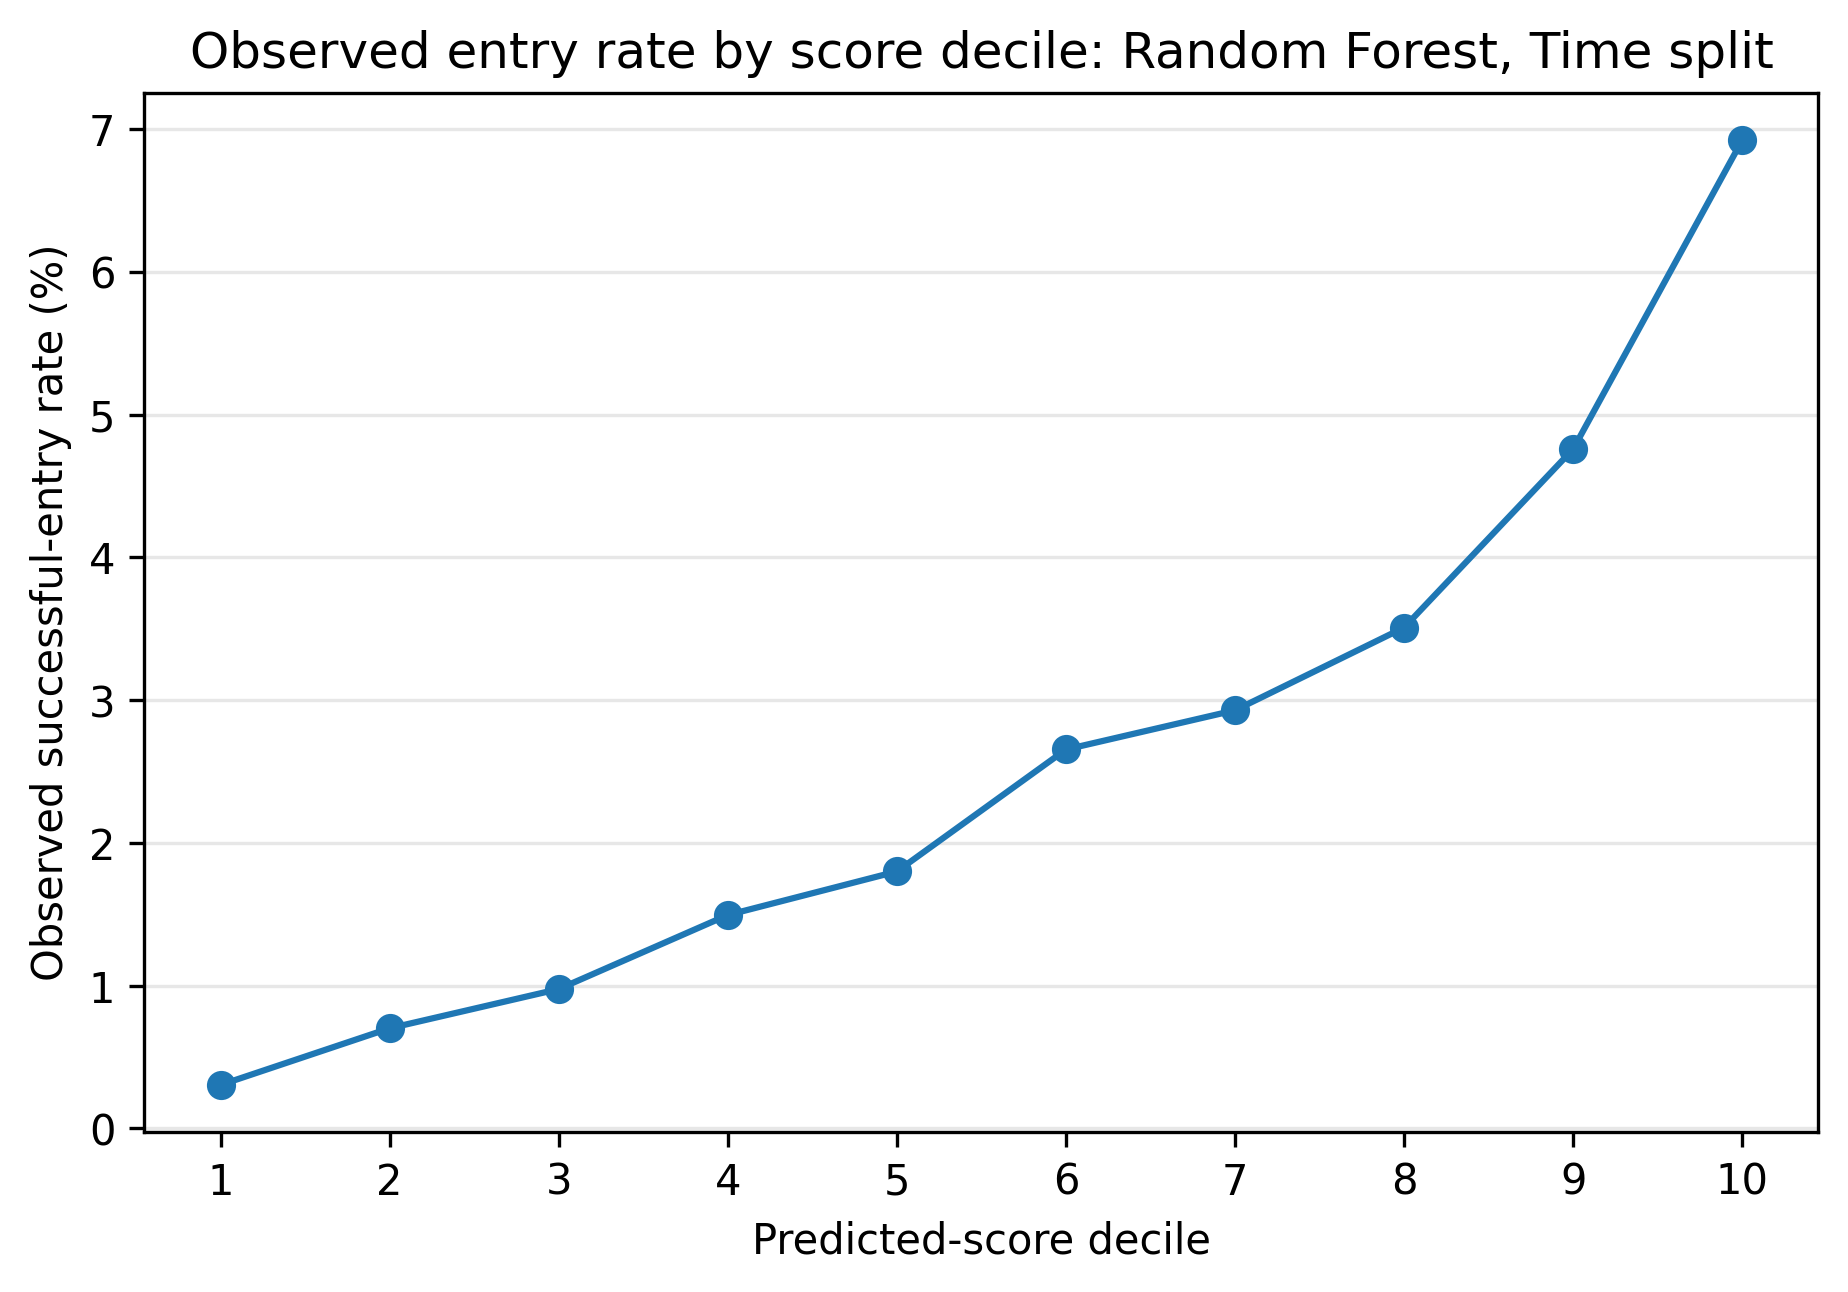
\includegraphics[width=12cm]{figures/fig_score_decile_random_forest_time}
\note{Note: The figure reports observed successful export-entry rates by decile of the Random Forest score in the main chronological test split.}
\end{figure}

\begin{figure}[!ht]
\caption{Targeting lift relative to simple policy rules} \label{fig:policy_lift}
\centering
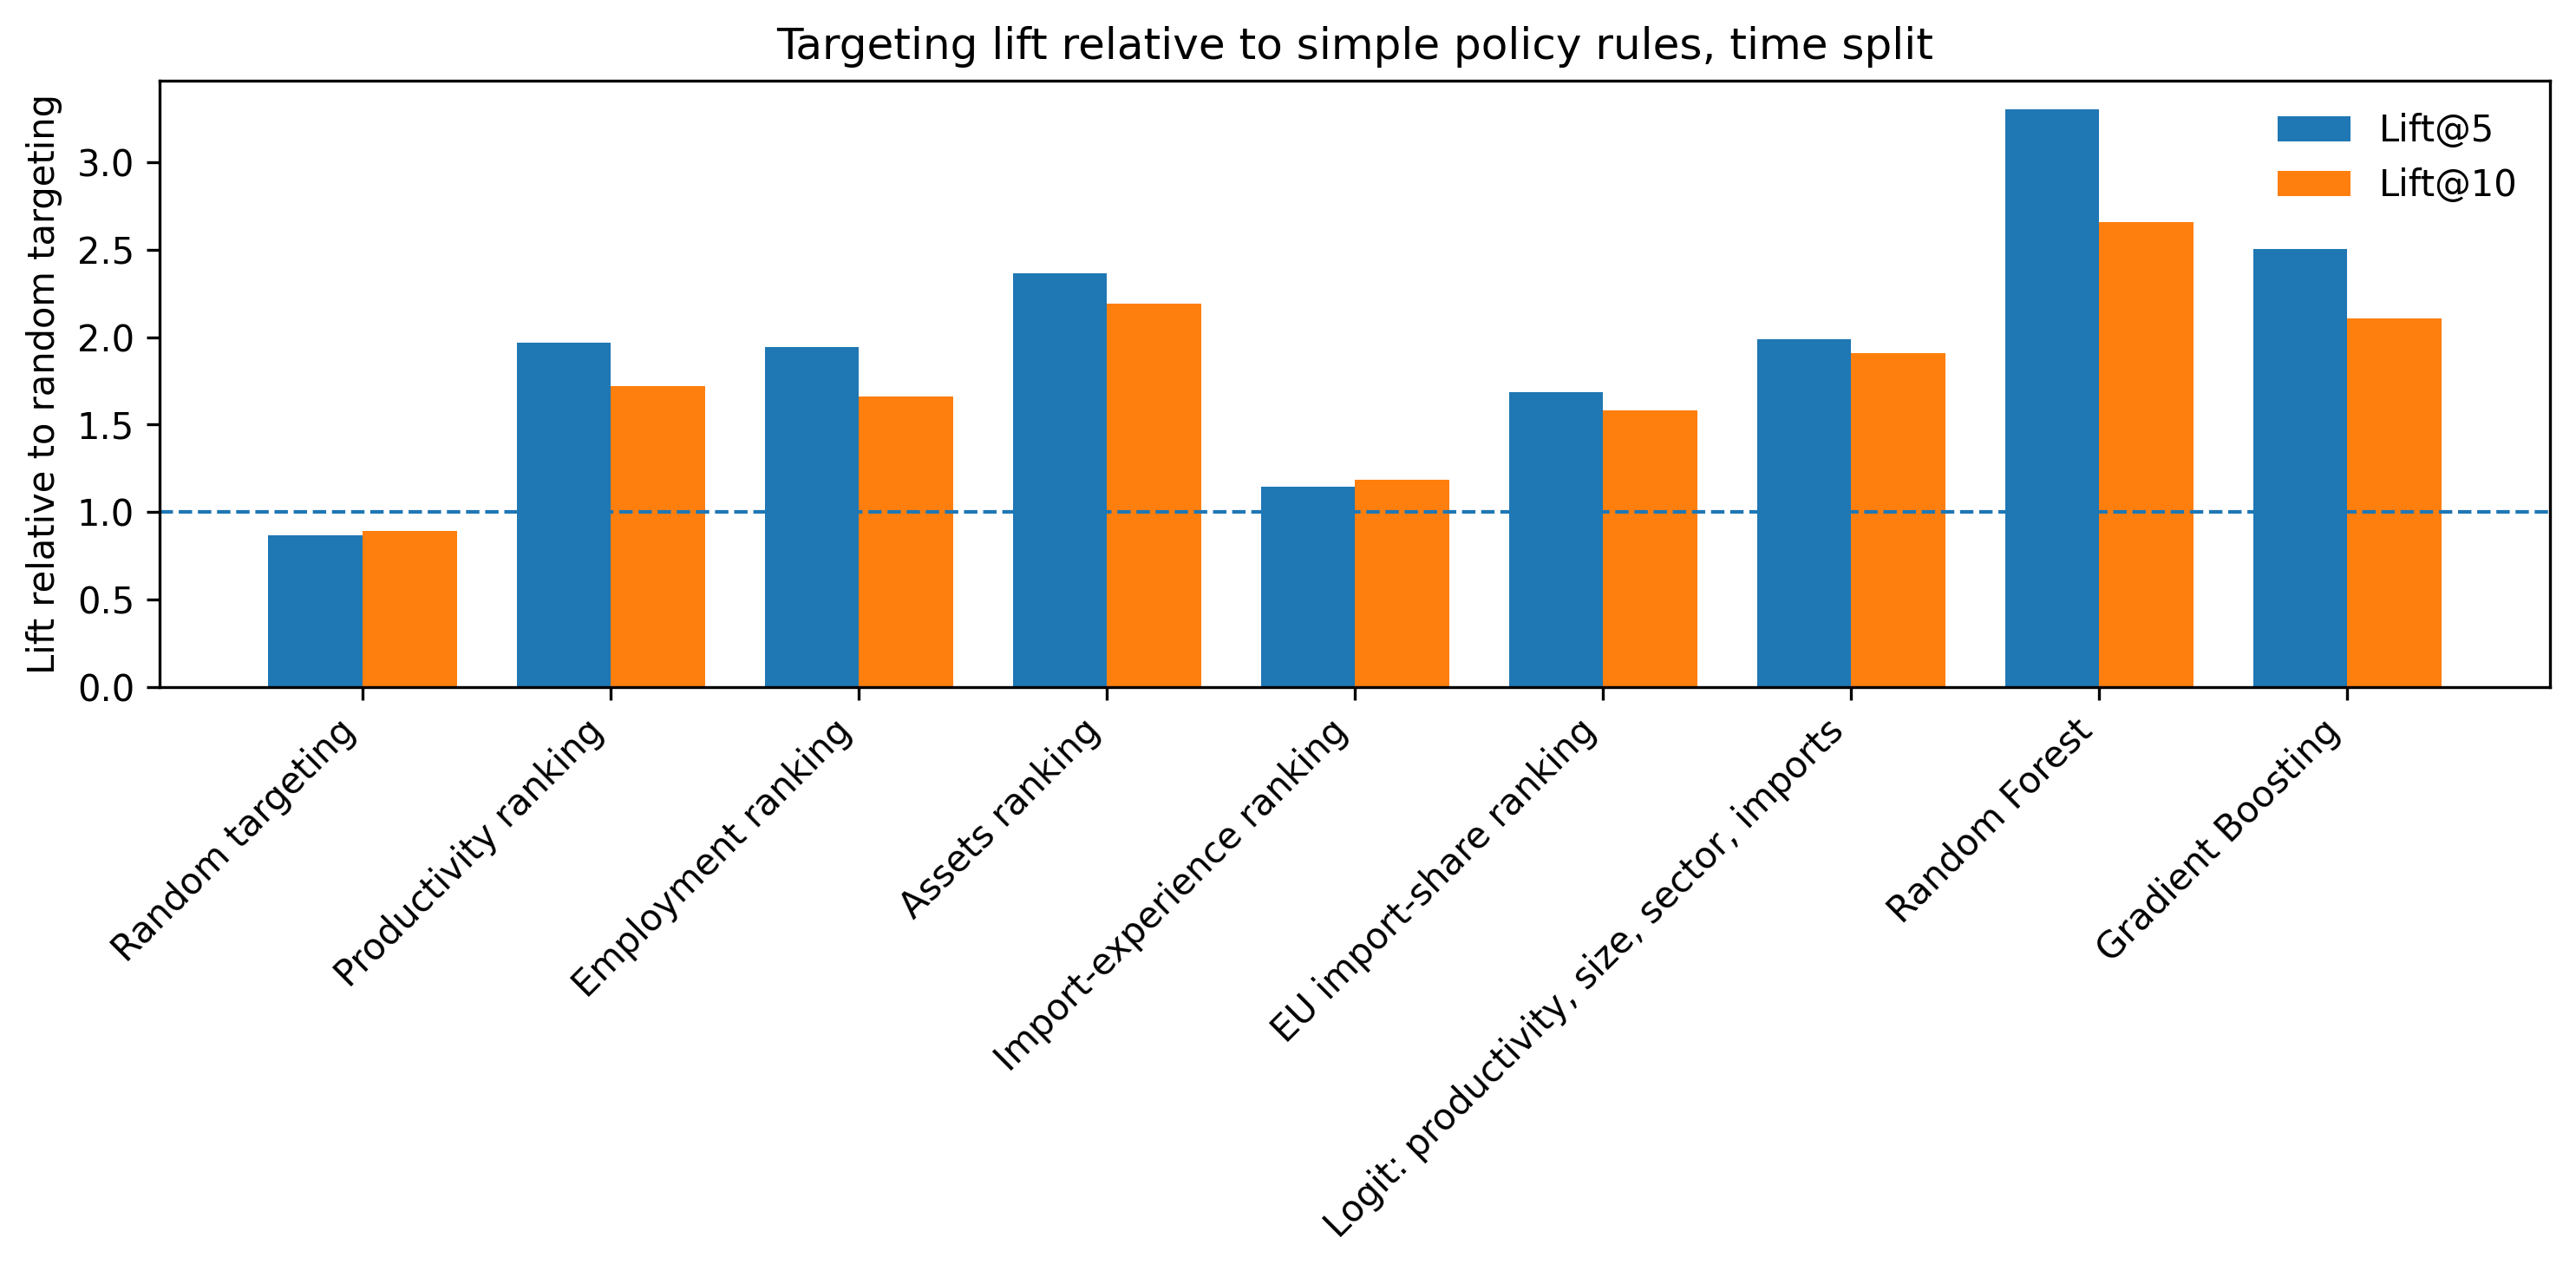
\includegraphics[width=12cm]{figures/fig_policy_lift_time}
\note{Note: The figure compares lift at the top 5\% and 10\% of the score distribution for simple rankings, policy-logit rules and model scores.}
\end{figure}

\begin{figure}[!ht]
\caption{Distribution of export-readiness scores by firm size} \label{fig:score_distribution_size}
\centering
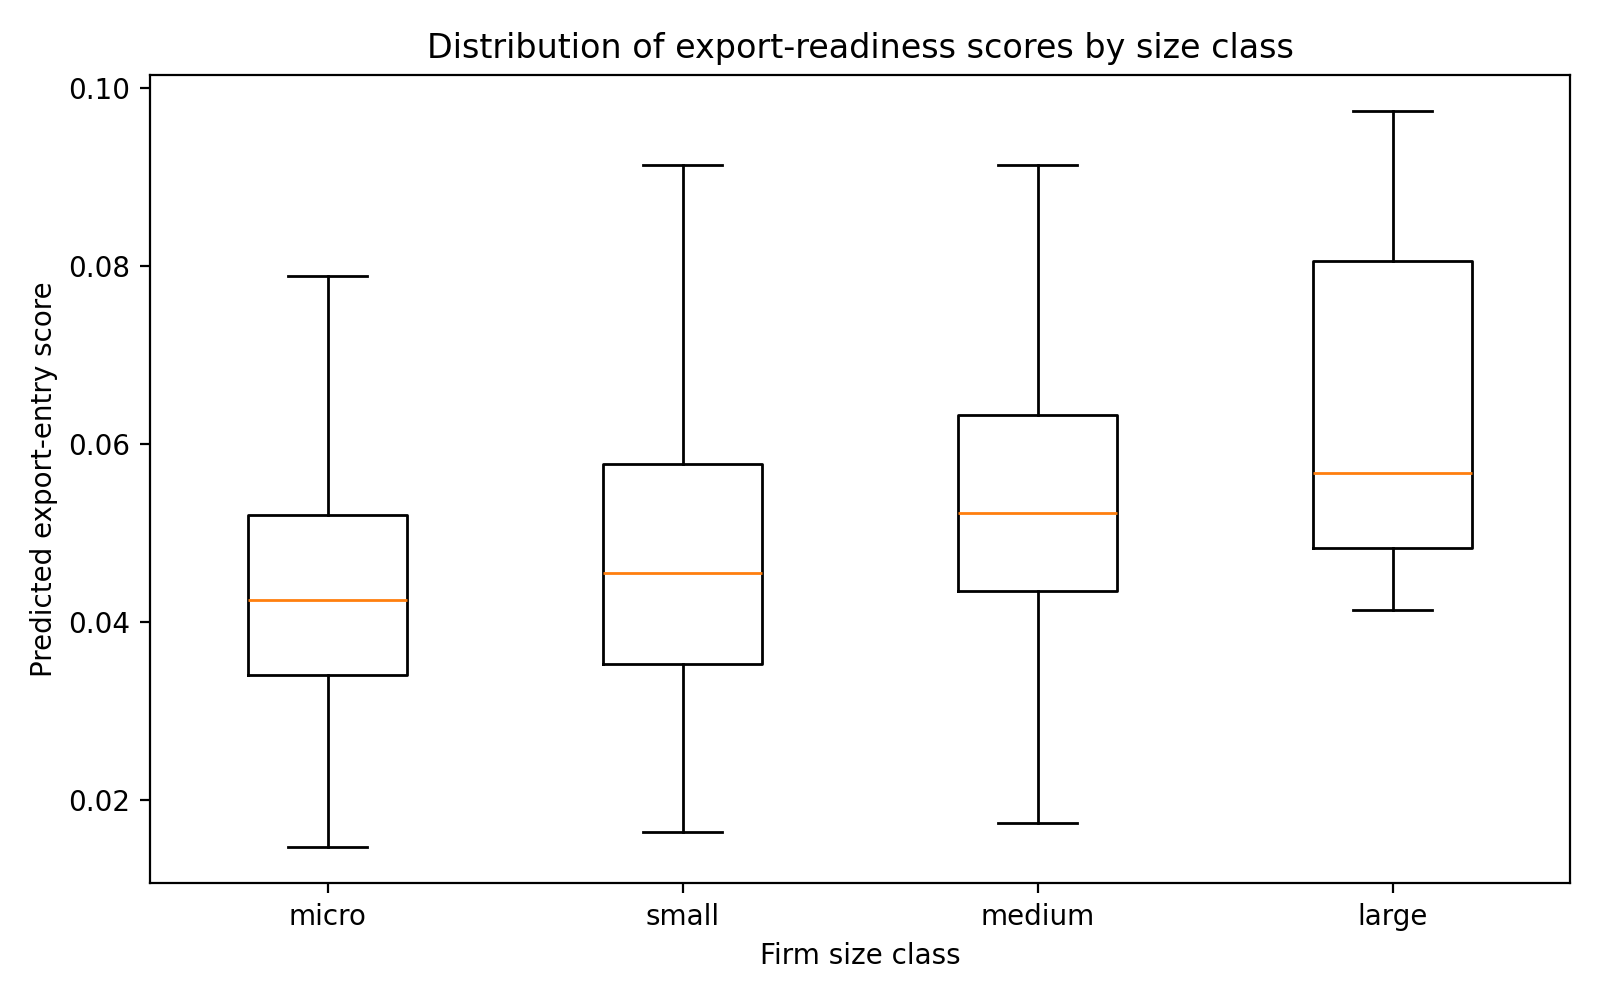
\includegraphics[width=12cm]{figures/fig_score_distribution_by_size}
\note{Note: The figure shows the distribution of predicted export-readiness scores across firm-size classes.}
\end{figure}

\begin{figure}[!ht]
\caption{Top-decile lift by firm-size group} \label{fig:size_lift}
\centering
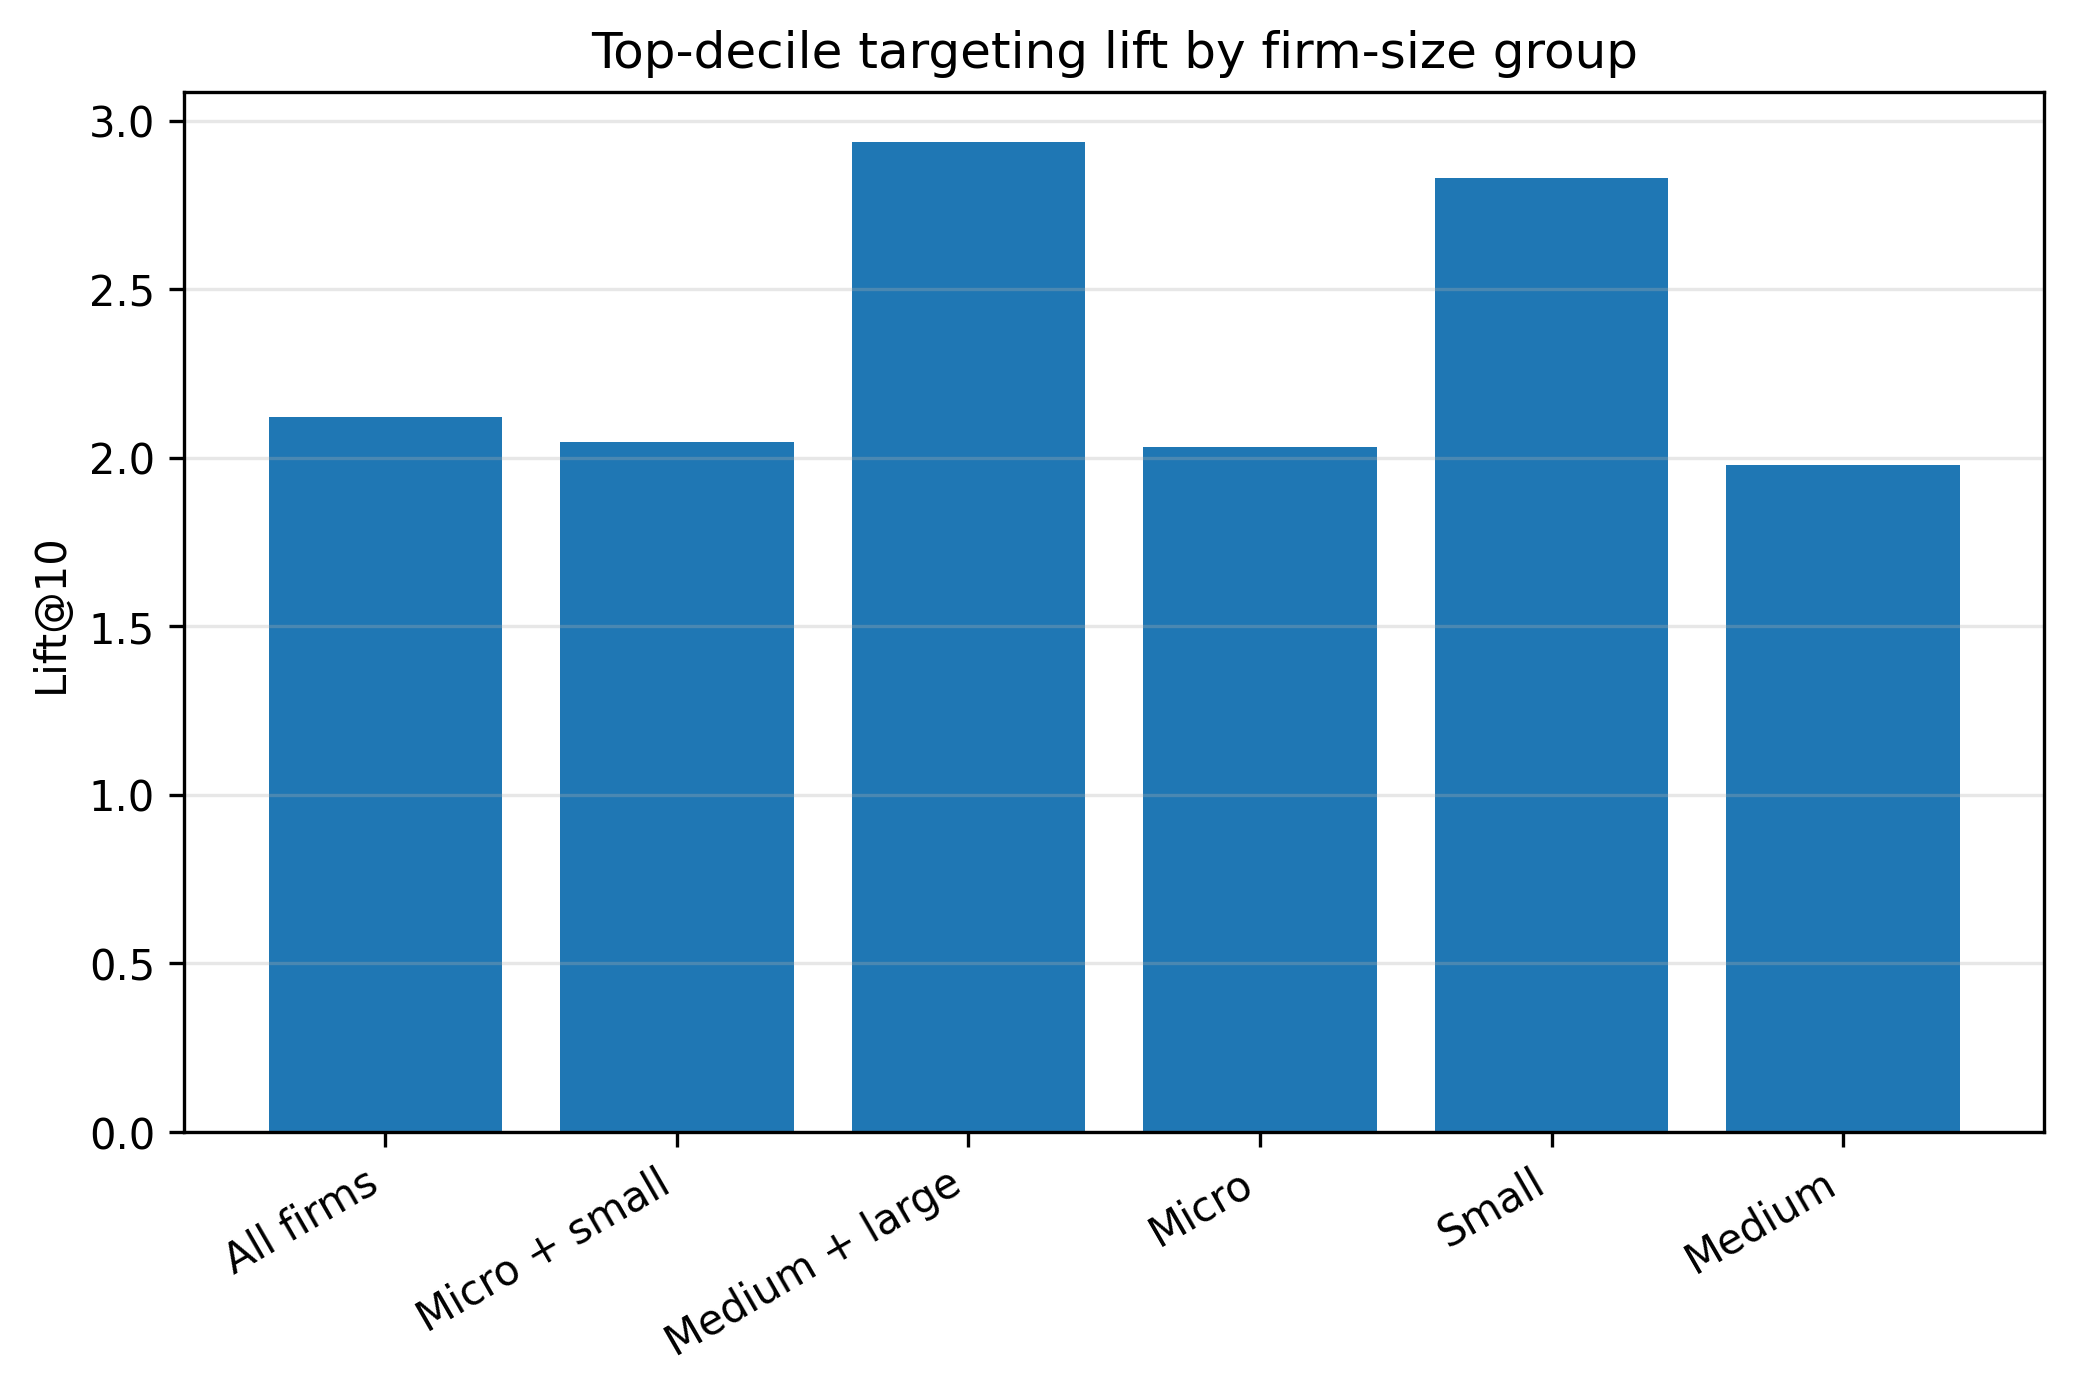
\includegraphics[width=12cm]{figures/fig_size_lift_at_10}
\note{Note: The figure reports lift at the top decile for models re-estimated within size groups.}
\end{figure}

\begin{figure}[!ht]
\caption{Predictive signals in the export-readiness score} \label{fig:perm_importance}
\centering
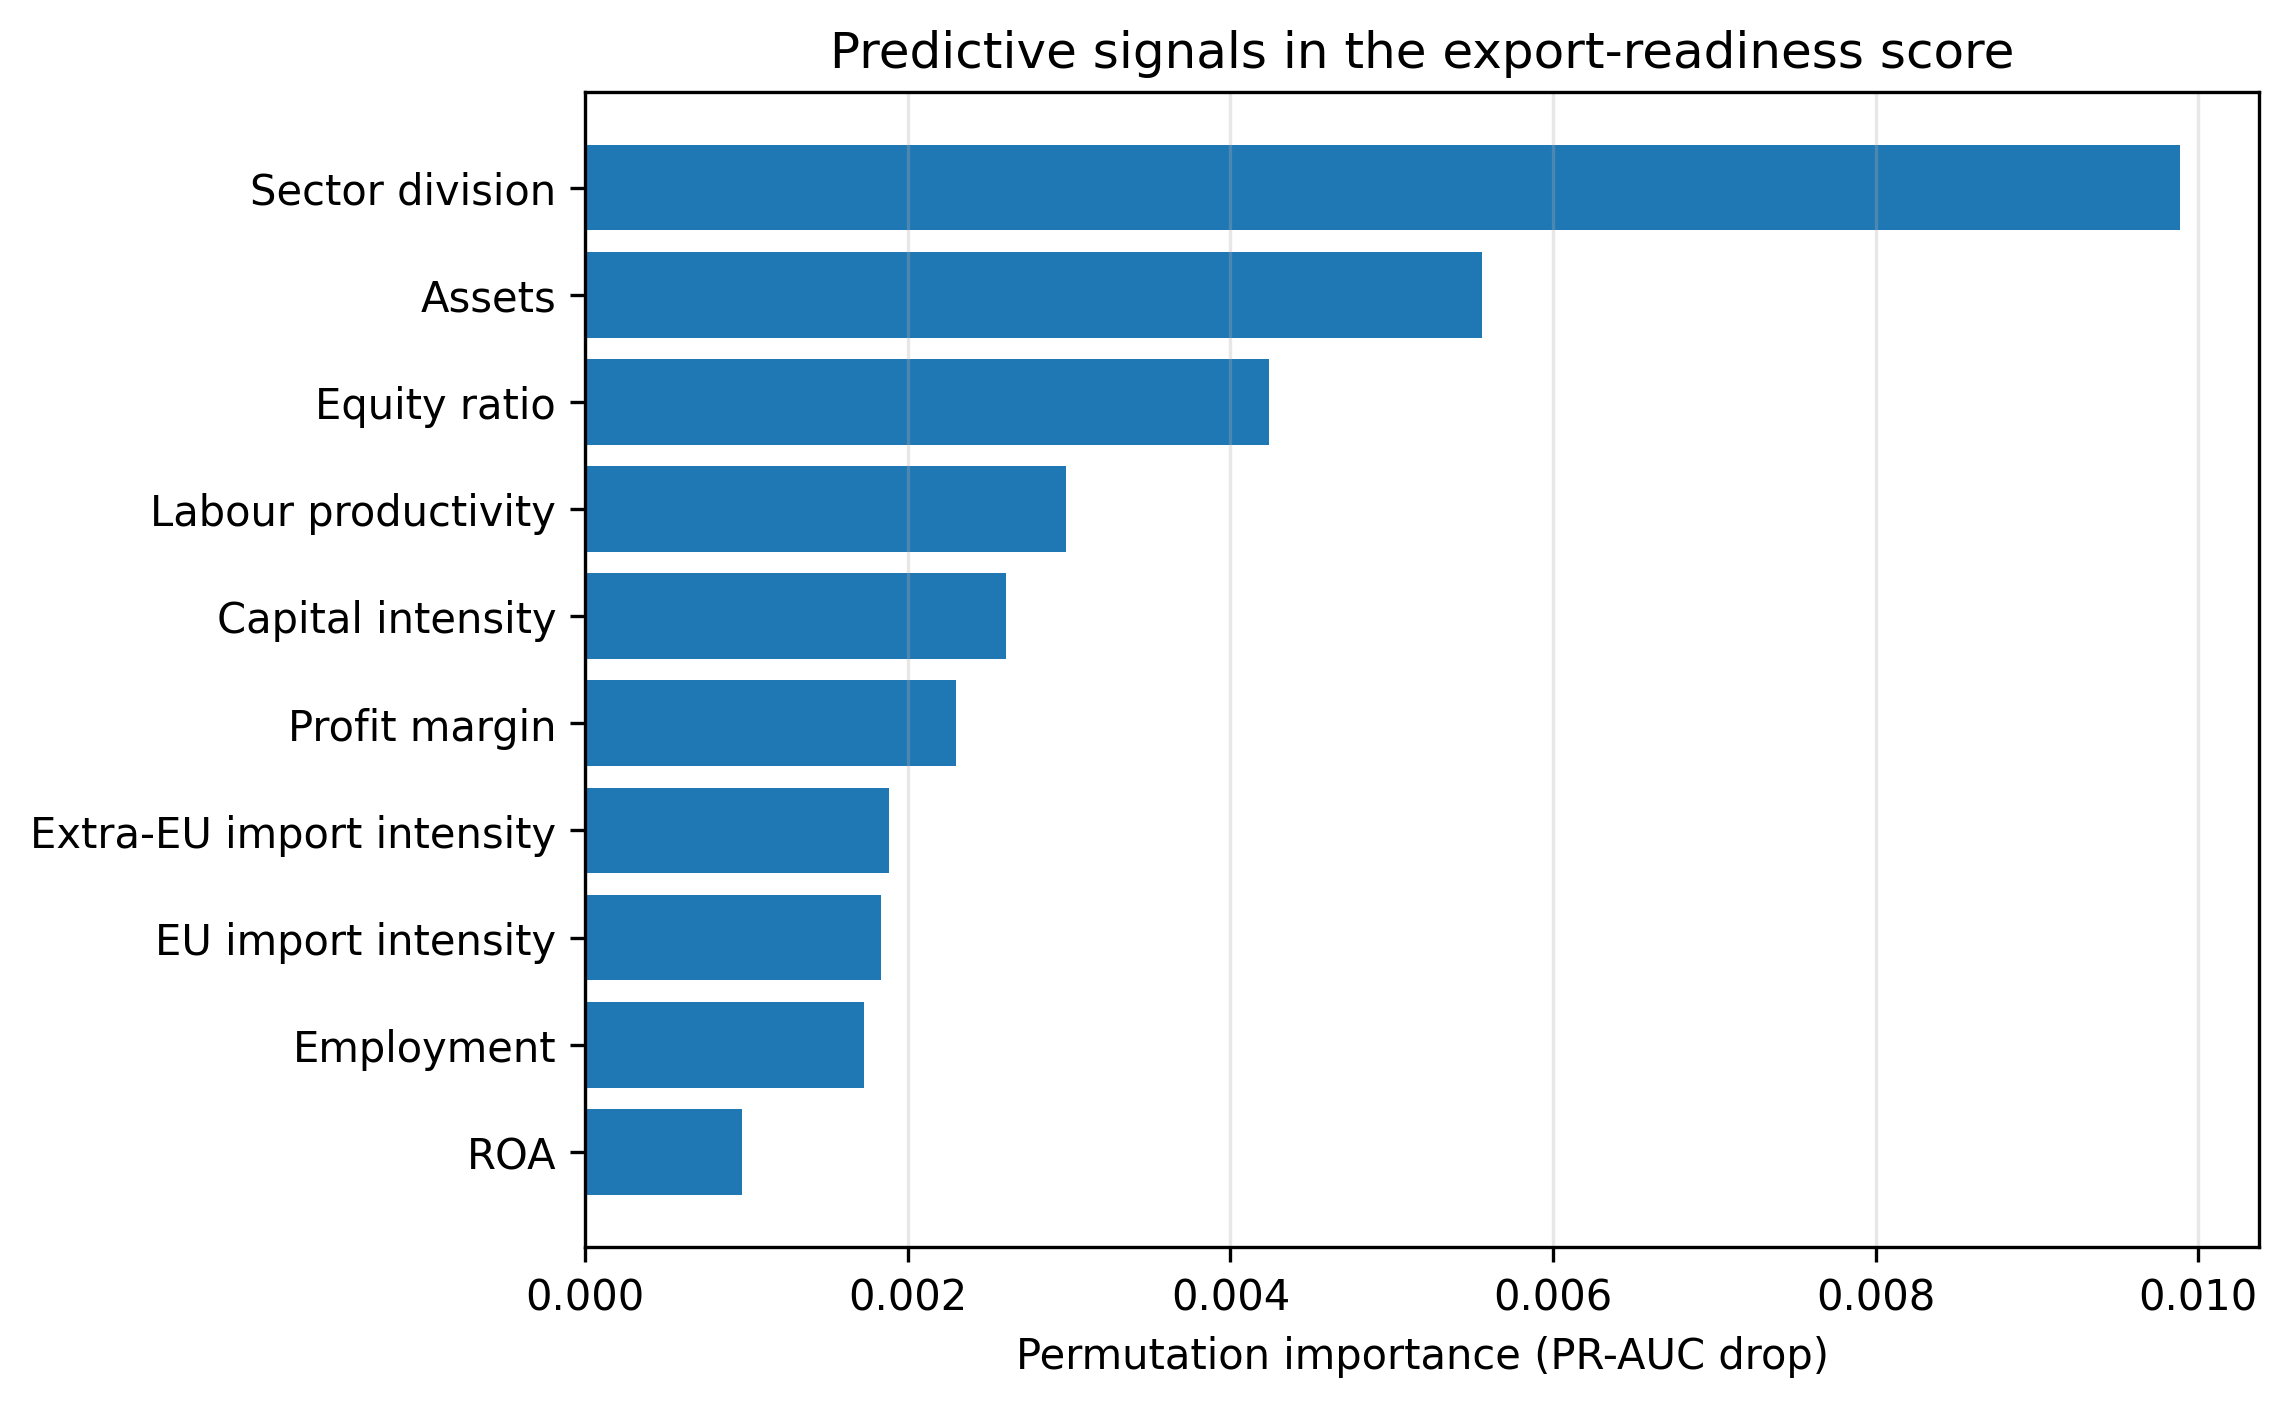
\includegraphics[width=12cm]{figures/fig_permutation_importance}
\note{Note: Permutation importance is computed on the test set using PR-AUC as the scoring metric. The estimates are predictive rankings, not causal effects.}
\end{figure}

\begin{figure}[!ht]
\caption{Candidate interaction pairs in export readiness} \label{fig:interaction_strength}
\centering
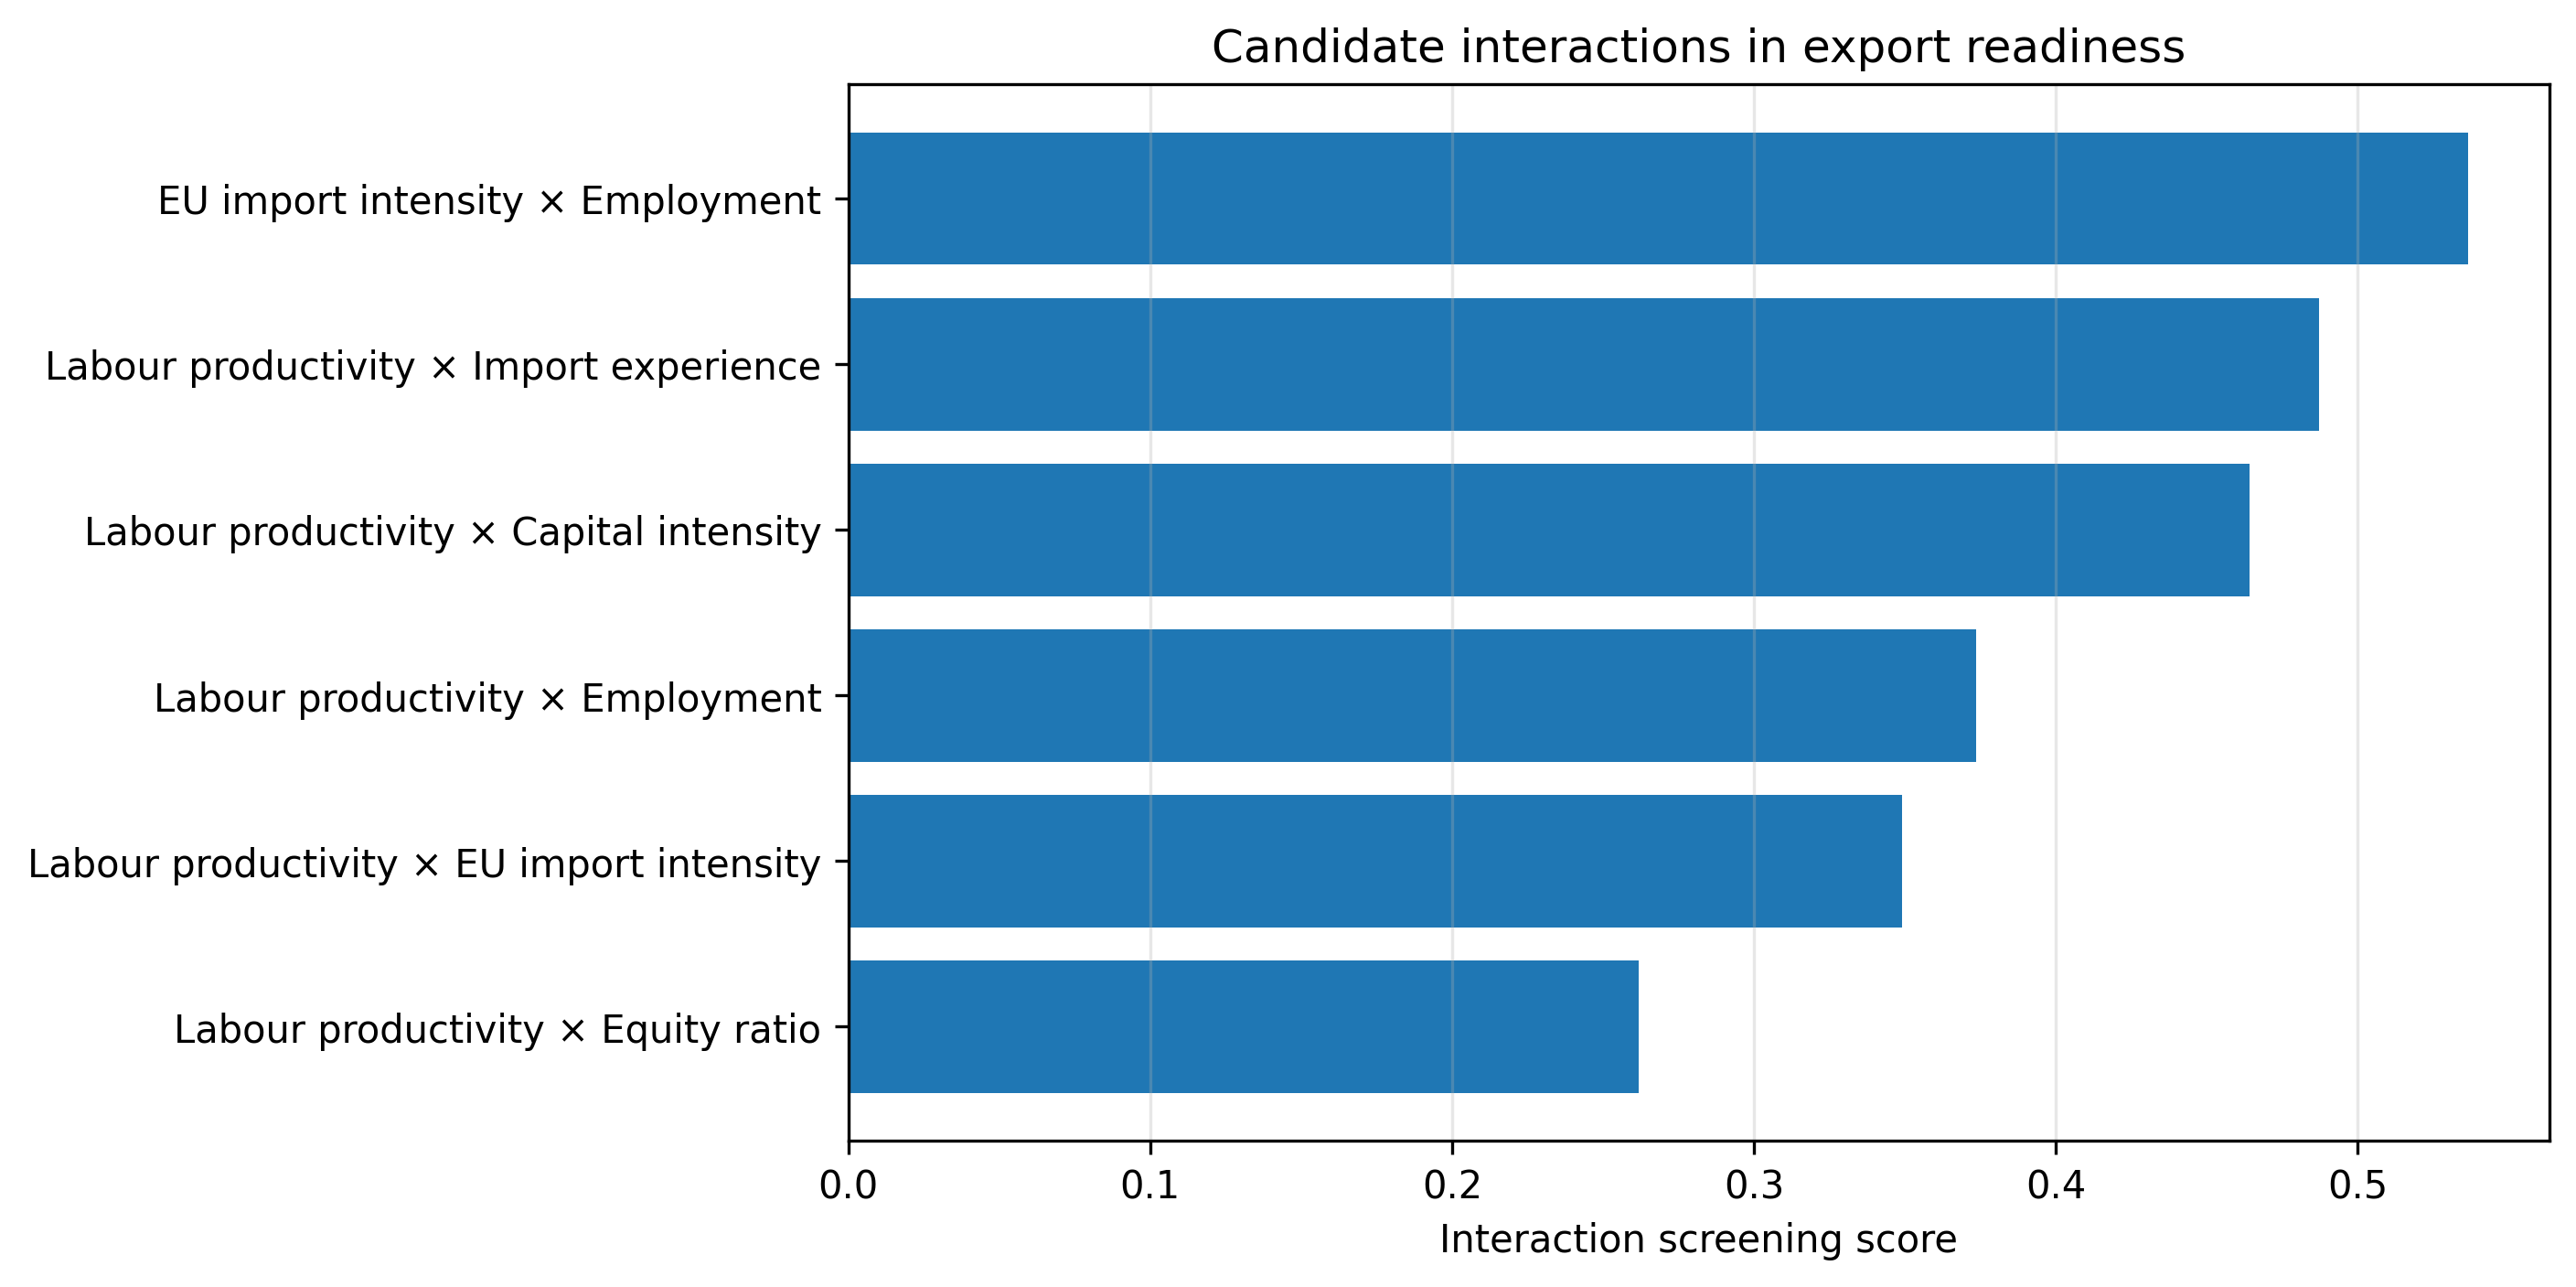
\includegraphics[width=12cm]{figures/fig_interaction_strength}
\note{Note: The figure ranks candidate interaction pairs used to select the partial-dependence or ALE plots in the main text and appendix.}
\end{figure}

% EC-style size-definition robustness (Appendix A): entrant composition + fixed-model regrouped lift
% AUTO-GENERATED by scripts/16_ec_size_comparison.py (v8, fixed-model regrouping).
% Outcome=entry_from_zero_to_success_t1; split=time; model=gradient_boosting. Do not edit by hand.
\begin{table}[!htbp]
\captionof{table}{Robustness of the entrant size composition and size-stratified lift to the size definition} \label{tab:ec_size_comparison}
\centering
\footnotesize
\setlength{\tabcolsep}{6pt}
\renewcommand{\arraystretch}{1.10}
\begin{tabular}{lcc}
\hline
\multicolumn{3}{l}{\textit{Panel A. Size composition of future successful entrants (main time-split test)}} \\
Size class & Employment-only & EC-style (headcount + turnover/assets) \\
\hline
Micro & 615 & 613 \\
Small & 201 & 201 \\
Medium & 35 & 37 \\
Large & 2 & 2 \\
Micro + small & 816 & 814 \\
\hline
Micro + small share (\%) & 95.7 & 95.4 \\
\hline
\multicolumn{3}{l}{\textit{Panel B. Top-decile lift by size group (single fixed model, regrouped)}} \\
Size group & Employment-only & EC-style (headcount + turnover/assets) \\
\hline
All firms & 2.11 [1.86, 2.36] & 2.11 [1.86, 2.36] \\
Micro + small & 2.03 [1.79, 2.36] & 2.03 [1.78, 2.31] \\
Micro & 2.00 [1.70, 2.33] & 1.99 [1.69, 2.33] \\
Small & 2.09 [1.56, 2.72] & 2.09 [1.54, 2.65] \\
Medium & 1.70 [0.62, 3.08] & 1.87 [0.76, 3.19] \\
\hline
\end{tabular}
\note{Note: A single Gradient Boosting model is trained once on the full candidate sample with the employment-only feature set, and its predictions are held fixed; only the size definition used to group firms changes across the two columns. The employment-only class is the one used as a model feature; the EC-style class follows the headcount bands of Recommendation 2003/361/EC together with the turnover-or-balance-sheet ceilings (turnover $=$ goods sales $+$ services), as a firm-level approximation that does not account for partner or linked enterprises. The main time-split test contains 854 entrants; Panel A reports the 853 entrants with a valid size classification (one entrant has missing size information). Among these 853 classified entrants, 849 (99.5\%) receive the same class under both definitions. Panel B reports top-decile lift within each size group, with 95\% firm-clustered bootstrap intervals. Because the model is held fixed and only regrouped, Panel B differs from Table~\ref{tab:size_ci}, which instead re-estimates a separate model within each size class.}
\end{table}

